% 2D Image with indices
% Author: Peter Steinbach
\documentclass[tikz]{standalone}
%\documentclass[dvisvgm]{standalone}
%\def\pgfsysdriver{pgfsys-tex4ht.def}
\usepackage{tikz}
\usepackage{units}
\usetikzlibrary{calc,trees,positioning,arrows.meta,chains,shapes.geometric,shapes.arrows,%
    decorations.pathreplacing,decorations.pathmorphing,shapes,%
    matrix,shapes.symbols,fit,backgrounds}

 \pgfdeclarelayer{back}
 \pgfsetlayers{background,back,main}


\makeatletter
\makeatother

\begin{document}


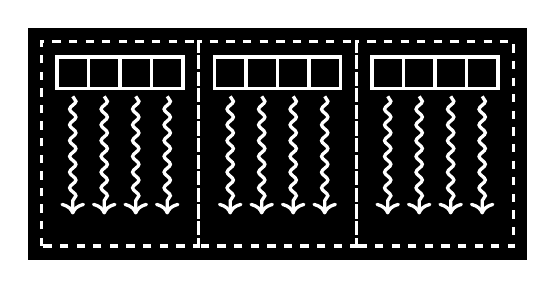
\begin{tikzpicture}[
  show background rectangle, 
  background rectangle/.style={fill=black},
  color=white,
  help lines/.style={color=lightgray,line width=.2pt},
  ]


  \foreach \g in {0,...,2}
  {
    
  \draw[very thick, dashed] ($(-.4,-.4)+(2*\g,0)$) rectangle ($(1.6,2.2)+(2*\g,0) $);

  \foreach \c in {0,...,3}
  {
  \draw[very thick] ($(-.2,1.6)+(.4*\c,0)+(2*\g,0)$) rectangle ($(.2,2.)+(.4*\c,0)+(2*\g,0)$);
  \draw [->,very thick,decorate, decoration={snake,amplitude=.4mm,segment length=2mm,post length=1mm}]  ($(0,1.5)+(.4*\c,0)+(2*\g,0)$) -- ($(0,0)+(.4*\c,0)+(2*\g,0)$);
}
}

\end{tikzpicture}
\end{document}
